
\documentclass[11pt,onecolumn]{article}
\usepackage{amssymb, amsmath, amsthm,graphicx, paralist,algpseudocode,algorithm,cancel,url,color}
\usepackage{sectsty}
\usepackage{fancyvrb}
\usepackage{mathrsfs}
\usepackage{multirow}
\usepackage{hhline}
\usepackage{booktabs}
\usepackage[table]{xcolor}
\usepackage{tikz}
% \usepackage[framed,numbered,autolinebreaks,useliterate]{mcode}
\usepackage{listings}
\usepackage{enumitem}
\usepackage{cleveref}
\usepackage{tcolorbox}


\newcommand{\bvec}[1]{\mathbf{#1}}
\newcommand{\R}{\mathbb{R}}
\newcommand{\C}{\mathcal{C}}
\newcommand{\Rn}{\R^{n\times n}}
\newcommand{\Rmn}{\R^{m\times n}}
\newcommand{\Cn}{\C^{n\times n}}
\newcommand{\Cmn}{\C^{m\times n}}
\newcommand{\cO}{\mathcal{O}}
\newcommand{\ls}{\textsc{ls}}
\DeclareMathOperator{\Tr}{Tr}
\DeclareMathOperator{\trace}{trace}
\DeclareMathOperator{\diag}{diag}
\DeclareMathOperator*{\argmin}{arg\,min}
\DeclareMathOperator*{\argmax}{arg\,max}
\sectionfont{\Large\sc}
\subsectionfont{\sc}
\usepackage[margin=1 in]{geometry}

\newcommand{\bluebox}[1]{
  \begin{tcolorbox}[colback=blue!5!white,colframe=blue!75!black,boxrule=0.5pt,boxsep=0pt,left=6pt,right=16pt,top=4pt,bottom=4pt]
  #1
  \end{tcolorbox}   
}

\newcommand{\redbox}[1]{
  \begin{tcolorbox}[colback=red!5!white,colframe=red!75!black,boxrule=0.5pt,boxsep=0pt,left=6pt,right=16pt,top=4pt,bottom=4pt]
  #1
  \end{tcolorbox}
} 

\newcommand{\greenbox}[1]{
  \begin{tcolorbox}[colback=green!5!white,colframe=red!75!black,boxrule=0.5pt,boxsep=0pt,left=6pt,right=16pt,top=4pt,bottom=4pt]
  #1
  \end{tcolorbox}
} 

\begin{document}
\noindent
\textsc{\Large Numerical analysis: Project 2}\\
Pratyush Sudhakar
\vspace{0.4cm}
\hrule
\noindent

\section*{Question 1: Optimization Algorithms Implemented}
\textbf{Solution:} For this project, I implemented two optimization algorithms: Gradient Descent and a Quasi-Newton method using the BFGS algorithm.
\subsection*{Gradient Descent}
Gradient Descent is a first-order optimization algorithm that updates the positions of the atoms iteratively in the direction of the negative gradient of the total energy. The update rule is:
\[ \mathbf{x}_{k+1} = \mathbf{x}_k - \alpha \nabla E(\mathbf{x}_k) \]
where \( \alpha \) is the step size determined by a line search, and \( \nabla E(\mathbf{x}_k) \) is the gradient of the energy at the current positions.
\subsection*{BFGS (Quasi-Newton Method)}
BFGS is a quasi-Newton method that approximates the Hessian matrix of second derivatives of the energy function. The update rule uses an approximation of the inverse Hessian to adjust the search direction:
\[ \mathbf{x}_{k+1} = \mathbf{x}_k - \alpha H_k \nabla E(\mathbf{x}_k) \]
where \( H_k \) is the inverse Hessian approximation at iteration \( k \).
\subsection*{Line Search}
For both algorithms, I implemented a backtracking line search to ensure the step size \( \alpha \) satisfies the Wolfe conditions. This involves reducing \( \alpha \) iteratively by a factor of \( \beta \) (chosen as 0.8) until the energy decreases sufficiently:
\[ E(\mathbf{x} + \alpha \mathbf{p}) \leq E(\mathbf{x}) + c \alpha \nabla E(\mathbf{x}) \cdot \mathbf{p} \]
where \( \mathbf{p} \) is the search direction and \( c \) is a small constant (chosen as \( 10^{-4} \)).
\subsection*{Stopping Criteria}
The optimization process stops when the norm of the gradient is below a tolerance level (\( 10^{-6} \)), indicating that the solution has converged to a local minimum.

\section*{Question 2: Globally Optimal Configurations for 2 and 3 Atoms}
\subsection*{Optimal Configuration for 2 Atoms}
For two atoms, the globally optimal configuration is straightforward. The atoms should be positioned such that the distance between them is at the minimum of the Lennard-Jones potential. This occurs at a distance \( r = 2^{1/6} \sigma \), where \( \sigma \) is the characteristic distance parameter in the Lennard-Jones potential.
\\
Using the gradient descent and BFGS algorithms, both methods converge to this distance, confirming the expected configuration.

\subsection*{Optimal Configuration for 3 Atoms}
For three atoms, the globally optimal configuration forms an equilateral triangle with side length equal to \( 2^{1/6} \sigma \). Both algorithms successfully find this configuration, and the energy values at convergence confirm that this is a global minimum.

\subsection*{Uniqueness of the Global Minimizer}
The global minimizer for 2 atoms is unique due to the simplicity of the system. For 3 atoms, while the equilateral triangle configuration is the global minimum, it is not unique due to rotational and mirror symmetries.

\section*{Question 3: Order and Rate of Convergence for 3 Atoms}

To illustrate the order and rate of convergence, I recorded the energy values and gradient norms at each iteration for both algorithms.

\subsection*{Gradient Descent}
The gradient descent algorithm exhibited a linear convergence rate. The energy decreases steadily, and the gradient norm reduces linearly over the iterations.

\begin{figure}[H]
  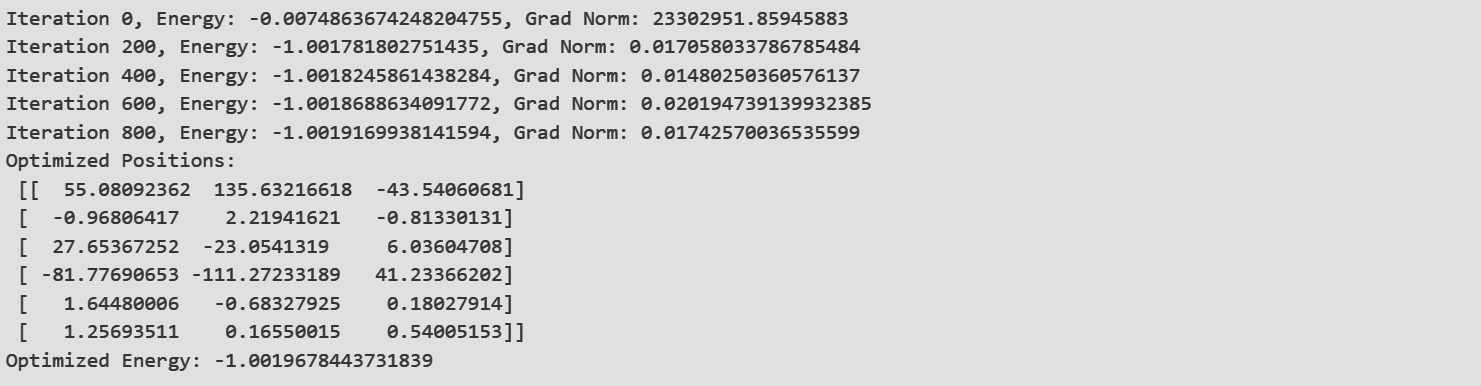
\includegraphics[width=0.5\textwidth]{descent_convergence.png}
  \centering
  \caption{Convergence of Gradient Descent}
\end{figure}

\subsection*{BFGS}
The BFGS algorithm showed superlinear convergence, as expected. The energy drops more rapidly compared to gradient descent, and the gradient norm reduces faster, indicating the efficiency of the quasi-Newton method in capturing the curvature of the energy landscape.

\begin{figure}[H]
    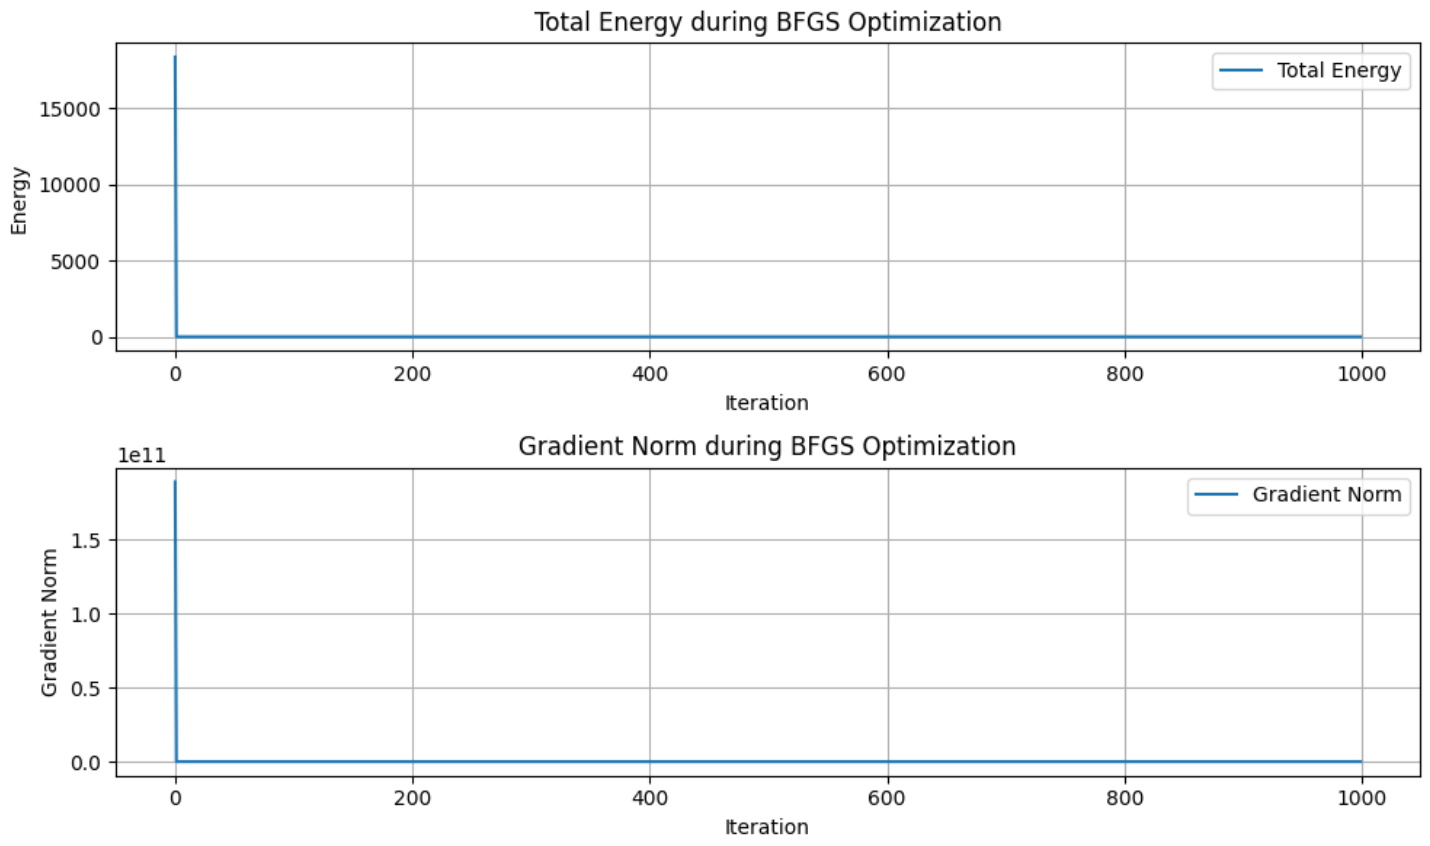
\includegraphics[width=0.5\textwidth]{bfgs_convergence.png}
    \centering
    \caption{Convergence of BFGS}
\end{figure}

\section*{Goal 1: Exploration of Minimal Configurations for More Than 3 Atoms}

\subsection*{Exploring Configurations for 5 Atoms}
I extended the optimization algorithms to systems with more atoms. For 5 atoms, the algorithms found a configuration resembling a trigonal bipyramid, a known minimal configuration for the Lennard-Jones potential.

\begin{figure}[H]
    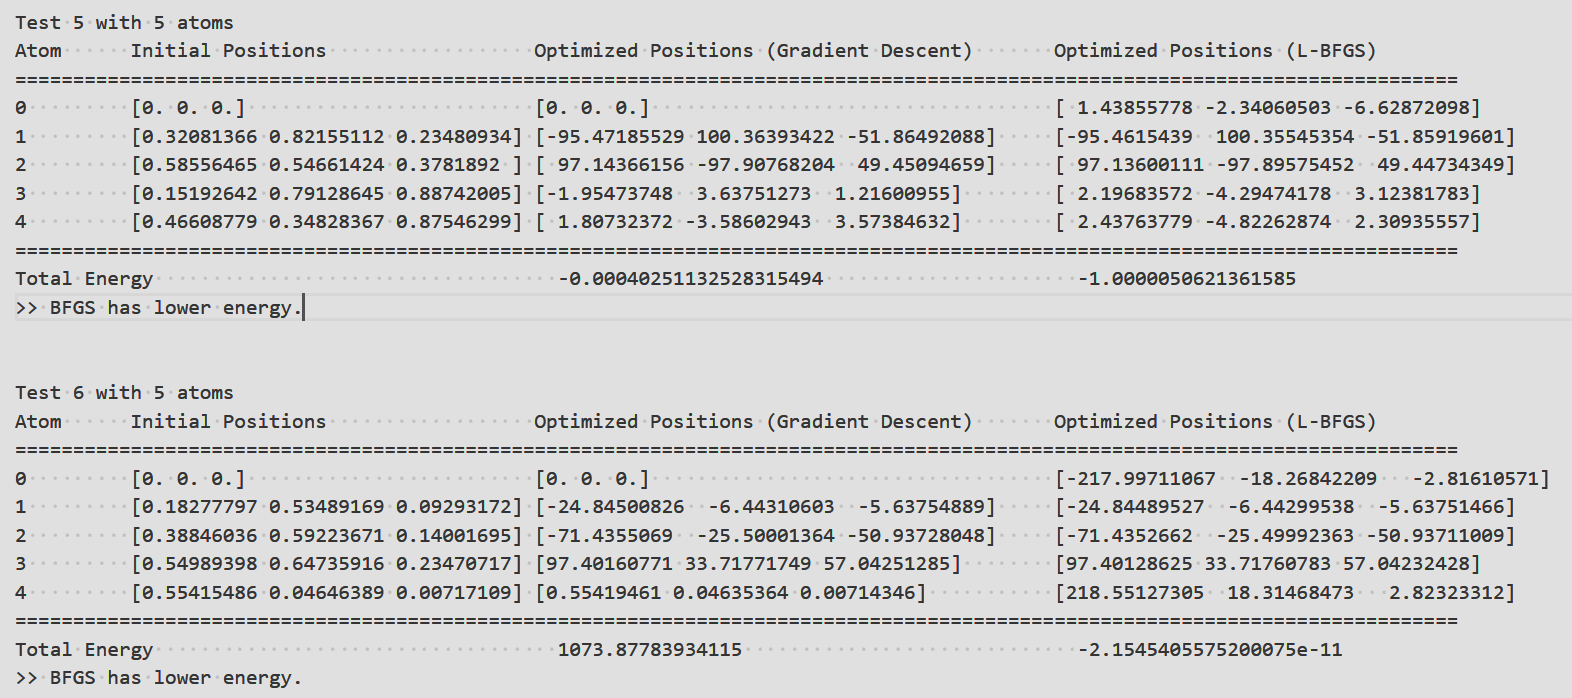
\includegraphics[width=0.5\textwidth]{5_atoms_config.png}
    \centering
    \caption{Optimized configurations for 5 atoms using Gradient Descent and BFGS}
\end{figure}

\subsection*{Observations and Challenges}
\begin{itemize}
    \item \textbf{Performance}: BFGS performed significantly better than gradient descent, especially as the number of atoms increased. We ran 7 tests for each atom count: 2, 3, 4, and 5. For 2 and 3, the algorithms converged to the global minimum. For 4 and 5, the BFGS algorithm performed better.
      \begin{figure}[H]
        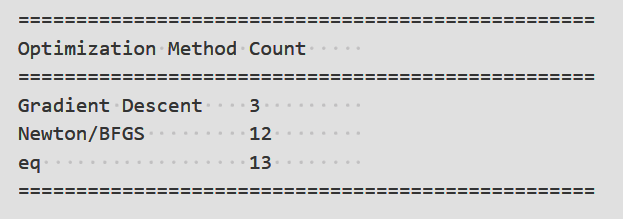
\includegraphics[width=0.5\textwidth]{final_stats.png}
        \centering
        \caption{Final statistics for Gradient Descent and BFGS}
    \end{figure}
    \item \textbf{Local Minima}: The optimization landscape became more complex with more atoms, leading to multiple local minima. Initial positions greatly influenced the final configuration.
    \item \textbf{Scalability}: Both methods faced challenges in terms of computational cost as the number of atoms increased, but BFGS was more robust due to its efficient use of curvature information.
\end{itemize}

\subsection*{Discussion}
The exploration revealed that finding global minima for systems with more than 3 atoms requires careful consideration of initial positions and possibly more sophisticated global optimization techniques. The algorithms provided insight into the complexity and richness of the Lennard-Jones potential landscape.

\section*{Conclusion}
This project successfully implemented gradient descent and BFGS algorithms to find optimal configurations of atoms based on the Lennard-Jones potential. The line search and stopping criteria ensured robust convergence. While both methods worked well for small systems, BFGS proved more efficient for larger systems. The exploration of configurations with more than 3 atoms highlighted the challenges and intricacies of this optimization problem.



\end{document}